% !Mode:: "TeX:UTF-8"
\chapter{需求分析}
上一章给出了虚拟漫游技术的研究意义与背景,本章将分析具体的需求,从而为后面的系统设计提供基础。

上一章中提到,传统的用于肠道疾病检测的内窥镜技术不仅对检查设备的操作技术要求较高,过程复杂且耗费时间,会给病人带来较大的痛苦,不便进行多次重复检查。为了给肠道疾病等需要使用内窥镜的疾病诊断提供一个更好的解决方案,为了更快更准确地检测疾病并且最大限度减少病人的负担,我们设计了本虚拟漫游系统。该系统的使用者是进行肠道疾病诊断的医生。

本系统是运行在装有Windows等操作系统的计算机上,通过接入CT扫描得到的图形资料,通过计算机进行图像分割,3D重建,中心路径提取等操作,生成漫游窗口供医生使用。
\section{功能需求}
本系统实现了从医学CT数据到虚拟漫游的全过程。主要包括以下功能:
\begin{enumerate}
    \item CT扫描图像导入
为了解决不同的CT机输出给计算机处理时相兼容的问题,医学图像有一个工业标准(医学数字图像和通信标准DICOM)。CT扫描生成的体数据是DICOM格式,该系统应该可以读取,显示,更改dicom格式的CT图像。除此此外还应该支持tif、bmp、raw等常见格式的图像。
    \item 大肠器官的提取及3D重建
为了实现虚拟漫游,必须从CT图像中分割出要观察的大肠,并且重建其3D模型。由于CT扫描输出的是一组图像,该系统需要对每个二维扫描面进行处理并将所有分离出来的大肠器官切片组合成3维模型,可以显示生成的3D模型,输出到特定格式的文件。
    \item 漫游路径生成
为了保证良好的漫游效果,需要计算机生成一个漫游的路径。并且可以在屏幕上用红色的线条表示出来。
    \item 虚拟漫游
该系统应该能渲染出器官模型并且可以使用鼠标滚轮或者键盘放大,缩小,能够用鼠标改变观察视角,能够用键盘实现前进,后退。
\end{enumerate}

系统用例图如\ref{use_case}所示:
\begin{figure}[h!]
    \centering
    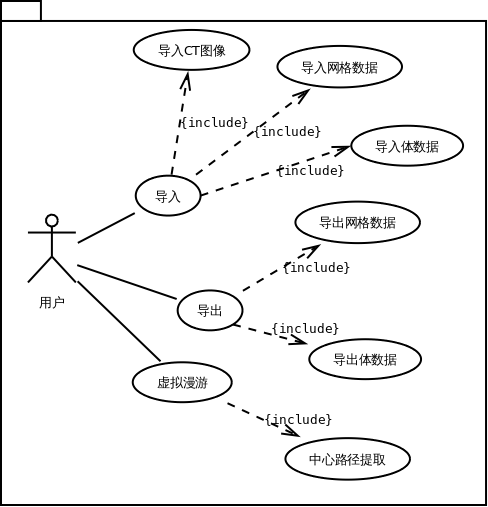
\includegraphics[width=400bp]{figure/use_case.png}
    \caption{系统用例图}
    \label{use_case}
\end{figure}

\section{性能需求}
对于导入,3D重建,漫游路径提取等功能,满足在可以接受的时间范围之内将数据处理出来即可,漫游功能必须实时响应用户的鼠标和键盘输入,为用户提供良好的操作体验。

\section{交互界面需求}
界面左边面板显示导入文件的信息,右边为显示区域可以显示渲染出来的器官模型或者漫游场景。菜单栏有导入,导出,生成中心路径,漫游等供选择。

\section{运行环境需求}
该系统运行在Windows XP/7平台上。

\section{本章小结}
本章对系统的需求进行了清晰的阐述,对于功能需求,采用了系统用例图方式进行了详细的描述与说明,可以作为指导系统设计的参考范例。
